\documentclass{report}

\usepackage{url}
\usepackage{indentfirst}
\usepackage{float}

\usepackage{xcolor, colortbl} % Used for coloring the cells of tables
\usepackage{amsmath}
\usepackage[T1]{fontenc}
\usepackage{textcomp} % Required for upquote.
\usepackage{listings} % Used for printing source code in papers

\usepackage{algorithm} % Used for writing algorithms in a paper
\usepackage[noend]{algpseudocode} % Allows psuedocode keywords (e.g. "if", "while", "for", etc.) in algorithms.

% Ensure quotes in listings are straight.
% Cleaner way to print strings in listings packages so no space symbol.
\lstset{showstringspaces=false, upquote=true} 

% eref puts parenthesis around reference, like "equation (1)"
\def\eref#1{(\ref{#1})}
% Used to generate || || (Norm) symbol for Paikin and Tal
\newcommand{\norm}[1]{\left\lVert#1\right\rVert}
\newcommand{\numbwithdegreesymbol}[1]{#1$^\circ$}

\DeclareMathOperator*{\argmax}{arg\,max} % The "*" means the limits go underneath "arg max"

% Used in the color of the table for Wrong Location
\definecolor{green}{rgb}{0,0.8,0}
\definecolor{red}{rgb}{1.0,0.0,0.0}
\definecolor{orange}{rgb}{1.0,0.6,0.2}
\definecolor{blue}{rgb}{0.0,0.0,1.0}


\usepackage{mdframed}
\usepackage[numbers,sort]{natbib}
%\usepackage[english]{babel} % Need for text wrap in table.
\usepackage{array} % Needed for centering in the table
\usepackage[export]{adjustbox} % loads also graphicx
\usepackage{graphicx}

\usepackage{hyperref} % Creates links in the PDF document.
\hypersetup{hidelinks} % Do not include boxes around links

% Defines the table of contents depth and the subsection numbering depth
\setcounter{secnumdepth}{5}
\setcounter{tocdepth}{5}

\title{An Enhanced Jigsaw Puzzle Solver \\[1in]
	   CS297 Final Report}

\author{
  Zayd Hammoudeh \\
  (zayd.hammoudeh@sjsu.edu)
  }


\newcommand{\myparagraph}[1]{\paragraph{#1}\mbox{}\\}

% Skip lines after each paragraph.
\setlength\parskip{\baselineskip}

\begin{document}

\maketitle

\pagenumbering{roman}

\renewcommand{\contentsname}{Table of Contents} % Change header of TOC from "Contents" to "Table of Contents"
\tableofcontents{\protect\newpage}

\addcontentsline{toc}{section}{List of Figures}
\listoffigures
\newpage

\addcontentsline{toc}{section}{List of Tables}
\listoftables
\newpage
 
\pagenumbering{arabic}

\renewcommand\thesection{\arabic{section}}

\section{Introduction}\label{sec:introduction}

Jigsaw puzzles have been around since the 1760s when they were made from wood.  Their name derives from the fact that they were originally carved using jigsaws.   The 1930s saw the introduction of the modern jigsaw puzzle where an image was printed on a cardboard sheet that was cut into a set of interlocking pieces \cite{williams1990, williams2004}.  Although jigsaw puzzles had been solved by children for centuries, it was not until 1964 that the first automated jigsaw puzzle solver was proposed by \cite{freeman1964}, and that solver could only solve 9 piece puzzles.  While an automated jigsaw puzzle solver may seem trivial, it has been shown by \cite{altman1990} and \cite{demaine2007} to be strongly NP-complete when pairwise compatibility between pieces is not a reliable metric for determining adjacency.

A jig swap puzzles are specific type of jigsaw puzzle where  all pieces are equally sized, non-overlapping squares.  Jig swap puzzles are substantially more difficult to solve than standard jigsaw puzzle as one can not consider mechanical compatibility when trying to determine affinity between pieces.  As such, one can only consider the image information on each individual piece when solving the puzzle.  

Solving a jigsaw puzzle simplifies to reconstructing an object from a set of component pieces.  As such, techniques developed for jigsaw puzzles can be generalized to many practical problems.  Examples where jigsaw puzzle solving strategies are applicable include: reassembly of archaeological artifacts \cite{brown2008, koller2006}, forensic analysis of deleted files \cite{garfinkel2010}, image editing \cite{cho2008}, reconstruction of shredded documents \cite{zhu2008}, DNA fragment reassembly \cite{marande2007}, and speech descrambling \cite{zhao2007}.

Unlike traditional jigsaw or jig swap puzzles, the ground-truth (i.e. original) image is unknown for most practical applications.  This significantly complicates solving the problem as one must determine the overall structure of the complete solution solely from a bag of individual pieces with unknown relationships.

This project proposes an improved jig swap puzzle solver.  It also studies the fundamental structures within images to determine which images are easy or difficult to solve using current techniques.  This study will help guide future research by focusing on the weaknesses with state of the art approaches. 

\pagebreak
\section{Previous Work}\label{sec:previousWork}

Computational solvers for jigsaw puzzles have been studied since the 1960s when Freeman and Garder proposed an approach that could solve jigsaw puzzles of up-to nine pieces using solely the piece shapes \cite{freeman1964}.  Since then the focus of research has shifted from traditional jigsaw puzzles to jig swap puzzles.  

Cho \textit{et. al.} \citep{cho2010} proposed in 2010 one of the first modern computational jig swap puzzle solvers; their approach relied on a graphical model build around a set of one or more ``anchor piece(s)''; these one or more anchor pieces were fixed in their correct location before the the solver began.  Cho \textit{et. al.} also assumed knowledge regarding the size of the puzzle dimensions.  Future solvers would on Cho \textit{et. al.}'s results while also reducing the amount of information passed to the solver beyond the set of pieces.

A significant contribution of Cho \textit{et. al.} is that they were first to use the LAB  (\underline{L}ightness and the \underline{A}/\underline{B} opponent color dimensions) colorspace to encode image pixels (as opposed to standards such as RGB or CMYK) since LAB normalizes the lightness and color variation across all three dimensions.  Cho \textit{et. al.} proposed a measure for quantifying the pairwise distance between two puzzle pieces that became the basis of most of the future work (see \ref{sec:piecePairwiseAffinity} for more details).  

Pomeranz \textit{et. al.} \cite{pomeranz2011} proposed an iterative, greedy jig swap puzzle solver in 2011.  Their solver did not rely on anchor pieces, and the only information passed to the solver were the pieces and the size of the puzzle.  Pomeranz \textit{et. al.} also generalized and improved on Cho \textit{et. al.} piece pairwise distance measure by proposing a ``predictive distance measure''.  Finally, Pomeranz \textit{et. al.} proposed the concept of ``best buddies'', which are two pieces that are more similar to each other than they are to any other pieces.  Best buddies have served as the basis for both an estimation metric for the quality of a solved image as well as the foundation of some solvers' placers \cite{paikin2015}.

An additional key contribution of Pomeranz \textit{et. al.} is the creation of three image benchmarks comprised of 20 images of 805 pieces drawn from \cite{mcgillImageDatabase} as well as images composed of 2,360 and 3,300 pieces.

In 2012, Gallagher \cite{gallagher2012} formalizes the different categories of jig swap problems into three primary types.  The following is Gallagher's proposed terminology, and his nomenclature is used throughout this document.

\begin{itemize}

	\item \textbf{Type 1 Puzzle}: The dimension of the puzzle (i.e. the width and height of the ground-truth image in number of pixels) is known.  What is more, the orientation of each piece is known, which means that there are exactly four pairwise relationships between any two pieces.  A single anchor piece, with a known, correct, location is required with additional anchor pieces being optional.  This type of puzzle is used by \cite{cho2010, pomeranz2011}.
	
	\item \textbf{Type 2 Puzzle}: This is an extension of a type 1, where pieces may be rotated in \numbwithdegreesymbol{90} increments (e.g. \numbwithdegreesymbol{0}, \numbwithdegreesymbol{90}, \numbwithdegreesymbol{180}, or \numbwithdegreesymbol{270}).  This change alone increases the number of possible solutions by a factor of $4^n$ (where $n$ is the number of pieces in the puzzles) in comparison to a Type 1 puzzle.  What is more, no piece locations are known in advance; this change eliminates the use of anchor piece(s).  Lastly, the dimensions of the ground-truth image/puzzle can be unknown.
	
	\item \textbf{Type 3 Puzzle}: All puzzle piece locations are known and only the rotation of the puzzle pieces is unknown.  This is the least computationally complex of the three puzzle variants and is generally considered the least interesting.  Type 3 puzzles are not explored as part of this thesis.

\end{itemize}

Sholomon \textit{et. al.} \cite{sholomon2013} in 2013 proposed a genetic algorithm based solver for type 1 puzzles.  By moving away from the greedy approached used by Pomeranz, Sholomon \textit{et. al.}'s approach is more immune to suboptimal decisions early in the placement process. Their approach is able to solve puzzles of significantly larger size than previous techniques (e.g. greater than 23,000) pieces.  What is more, Sholomon \textit{et. al.} provided a new benchmark of images of varying difficulty with 5,015, 10,375, and 22,834 pieces \cite{sholomonBenchmarkImages}.

Paikin \& Tal \cite{paikin2015} in 2015 published a greedy solver that can handle type 1 and type 2 images.  What is more, their solver is able to handle puzzles with missing; it can also solve multiple puzzles simultaneously.  Their solver is explored in significant depth in Section\ref{sec:paikinTalSolver}.














%%%%%%%%%%%%%%%%%%%%%%%%%%%%%%%%%%%%%%%%%%%%%%%%%%%%%%%%%%%%%%%%%
%              Puzzle Piece Pairwise Affinity                   %
%%%%%%%%%%%%%%%%%%%%%%%%%%%%%%%%%%%%%%%%%%%%%%%%%%%%%%%%%%%%%%%%%

\pagebreak
\section{Puzzle Piece Pairwise Affinity}\label{sec:piecePairwiseAffinity}

Pairwise affinity quantifies the similarity between the edges of two puzzle pieces.  $D(x_i, s_i, x_j, s_j)$ and $C(x_i, s_i, x_j, s_j)$ represent the distance and compatibility (i.e. similarity) between side $s_i$ of puzzle piece $x_i$ and side $s_j$ of puzzle piece $x_j$.  

\subsection{Cho \textit{et. al.} Pairwise Affinity}\label{sec:choPairwiseAffinity}

As mentioned in section \ref{sec:previousWork}, Cho \textit{et. al.} \cite{cho2010} proposed one of earliest edge-based pairwise affinity measures for two puzzle pieces.  Their approach is shown in Equation~\eref{eq:choPairwise}, which quantifies the distance between the left (``$L$'') side of piece $x_i$ and the right (``$R$'') side of piece $x_j$.  $K$ is the width/height of a puzzle piece in number of pixels\footnote{Cho \textit{et. al.} used 7 for $K$.}.  

\begin{equation} \label{eq:choPairwise}
D(x_i,L,x_j,R) = \sum_{k=1}^{K}\sum_{d=1}^{3}(x_i(k,K,d) - x_j(k,1,d))^2
\end{equation}

Since the LAB colorspace has three dimensions (e.g. lightness and A/B opponent colors), $d$ ranges between $1$ and $3$.  Similarly, $x_i(k,K,d)$ represents the LAB value in dimension $d$ of the pixel in row ``$k$'' of column $K$ in piece $x_i$.

\subsection{Pomeranz \textit{et. al.} Pairwise Affinity}\label{sec:pomeranzPairwiseAffinity}

One of the disadvantages of Cho \textit{et. al.}'s metric is that it simply squares the difference between the piece's pixel dimensions.  It is possible that superior results may be achieved by allowing the solver to modify this exponent term.  Pomeranz \textit{et. al.} in \cite{pomeranz2011} generalize Equation~\eref{eq:choPairwise} using the $L_p$ norm as shown in Equation~\eref{eq:pomeranzPairwise}\footnote{Pomeranz \textit{et. al.} used 28 for $K$.  This has generally become the standard in subsequent papers.}.

\begin{equation} \label{eq:pomeranzPairwise}
D(x_i,L,x_j,R) = \bigg(\sum_{k=1}^{K}\sum_{d=1}^{3}(|x_i(k,K,d) - x_j(k,1,d)|)^p\bigg)^{\frac{q}{p}}
\end{equation}

Hence, for a distance measure equivalent to that of Cho \textit{et. al.}, $p$ and $q$ are set equal to $2$.

An additional down side of the metric proposed by Cho \textit{et. al.} is that it only considers the border pixels.  Hence, if there is some gradient in the ground-truth image, two pieces may appear artificially dissimilar using this approach.  To address this issue, Pomeranz \textit{et. al.} proposed predictive compatibility.  Equation~\eref{eq:pomeranzPredCompat} shows the predictive compatibility between the left (``$L$'') side of piece $x_i$ and the right (``$R$'') side of piece $x_j$.  

\begin{equation} \label{eq:pomeranzPredCompat}
\begin{split}
C(x_i,L,x_j,R) = \sum_{k=1}^{K}\sum_{d=1}^{3}\Big[ ([2x_i(k, K, d) - x_i(k, K-1, d)] - x_j(k, 1, d))^p \\ - ([2x_j(k, 1, d) - x_i(k, 2, d)] - x_i(k, K, d))^p\Big]^{\frac{q}{p}}
\end{split}
\end{equation}

Note that in Equation~\eref{eq:pomeranzPredCompat}, the difference between the column of pixels adjacent to the edge is used to account for any gradient effects.

\subsection{Paikin \& Tal Pairwise Affinity}\label{sec:paikinPairwiseAffinity}

Paikin \& Tal in \cite{paikin2015} used Pomeranz \textit{et. al.}'s predictive compatibility as the foundation of their asymmetric distance measure.  Paikin \& Tal's approach is shown in Equation~\eref{eq:paikinAsymDistance}.

\begin{equation} \label{eq:paikinAsymDistance}
D(x_i,L,x_j,R) = \sum_{k=1}^{K}\sum_{d=1}^{3} \norm{[2x_i(k, K, d) - x_i(k, K-1, d)] - x_j(k, 1, d)}
\end{equation}

Note that Paikin \& Tal set $p$ and $q$ equal to 1 as it not only increased the accuracy of the solver but also significantly reduced the computational time.  It is important to note that since this distance is asymmetric, in most cases $D(x_i,L,x_j,R)$ will not equal $D(x_j,R,x_i,L)$.

Pomeranz \textit{et. al.} only considered the relationship between two individual pieces when determining the pairwise compatibility.  In images (or areas of images) with little variation (e.g. an all white image), parts may have artificially high pairwise distances.  To account for this, Paikin \& Tal proposed asymmetric compatibility as shown in Equation~\eref{eq:paikinAsymCompatibility}.

\begin{equation} \label{eq:paikinAsymCompatibility}
C(x_i,L,x_j,R)=1 - \frac{D(x_i,L,x_j,R)}{secondD(x_i,L)}
\end{equation}

\noindent
where $secondD(x_i,L)$ is the second best asymmetric distance between the left side of piece $x_i$ and all other pieces.  By normalizing compatibility with respect to the second best match, it is possible to identify those pairings that have actually have high compatibility while at the same time removing the artificially high compatibilities between pieces from areas of the image with low variation.

\subsubsection{Improved Asymmetric Compatibility}\label{sec:hammoudehPairwiseAffinity}

In an image that was generated from an analog input (e.g. a photograph), it is expected that there will be some degree of natural variation across the image due to variations in brightness, the object in the photo, and the image sensor.  However, in digital images that are generated or manipulated by computers, this variation can be trivially removed.  An example of this would be an image of a solid color or object(s) in front of a white background as shown in figure~\ref{fig:objectWhiteBackground}.

\begin{figure}
\centering
\fbox{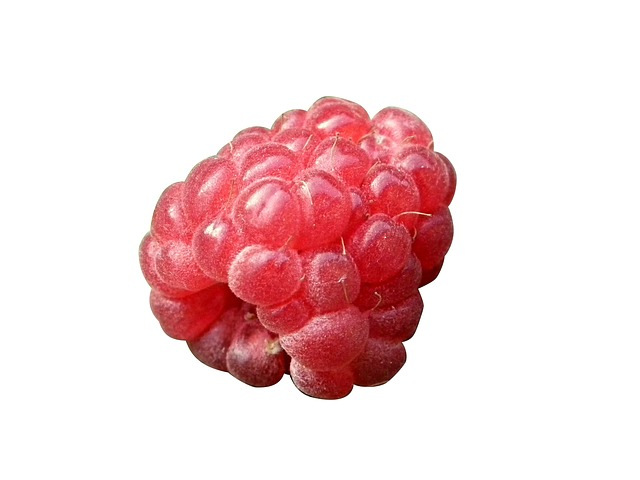
\includegraphics[width=50mm]{./images/raspberry_pixabay.jpg}}
\caption{A Computer Manipulated Image with Poor Asymmetric Compatibility}
\label{fig:objectWhiteBackground}
\end{figure}

The puzzles pieces along the border of the image as well as the pieces in the background have sides that are all white.  This entails that regardless of which of the three metrics are used, the distance between them is zero.  What is more, Paikin \& Tal do not explicitly define how to handle this case for asymmetric compatibility.  Therefore, to better handle computer generated images, this thesis proposes an enhanced definition of asymmetric compatibility as shown in Equation~\eref{eq:hammoudehAsymCompatibility}.  

\begin{equation} \label{eq:hammoudehAsymCompatibility}
C(x_i,L,x_j,R)= \begin{cases} 
	1 - \frac{D(x_i,L,x_j,R)}{secondD(x_i,L)} & secondD(x_i,L) \ne 0
\\
	-\alpha & secondD(x_i,L) = 0
\end{cases} 
\end{equation}

\noindent
where $\alpha$ is a penalty term that denotes that such pairings have low compatibility.


\subsection{Best Buddies}\label{sec:bestBuddies}

As defined by Pomeranz \textit{et. al.}, two pieces, $x_i$ and $x_j$ are best buddies on their respective sides $s_i$ and $s_j$ if they are more compatible (i.e. similar) to each other than they are to each other.  This is more formally described in Equation~\eref{eq:bestBuddyDefinition}.  This definition of best buddies applies regardless of whether the compatibility definition of Pomeranz \textit{et. al.} or Paikin \& Tal is used.

\begin{equation} \label{eq:bestBuddyDefinition}
\begin{split}
\begin{matrix}
\forall{x_k} \forall{s_k} \in Parts, & C(x_i, s_i, x_j, s_j) \geq C(x_i, s_i, x_k, s_k)
\\
\\
\multicolumn{2}{c}{\textnormal{and}}
\\
\\
\forall{x_k} \forall{s_k} \in Parts, & C(x_j, s_j, x_i, s_i) \geq C(x_j, s_j, x_k, s_k)
\end{matrix}
\end{split}
\end{equation}

\noindent
$Parts$ represents the set of all pieces in the puzzle, and $s_k$ is any of the four sides of piece $x_k$.

In most cases, it is relatively rare that two pieces are best buddies and are not actually neighbors \cite{paikin2015}.  When considering all sides of a piece, it is rarer still that a piece has more best buddies that are not its neighbor than that are its neighbor.  This makes best buddies a critical tool in many placers.

\subsubsection{Visualizing Best Buddies}\label{sec:visualizingBestBuddies}

There is currently no standard for visualizing best buddy relationships in images.  This thesis proposes a format for the first time.  As a nomenclature, this thesis refers to any best buddies that are neighbors in the image as ``adjacent best buddies'' while any best buddies that are not neighbors are referred to as ``non-adjacent best buddies''.  

In a jig swap puzzle, a piece may have best buddies on up to four sides (since the pieces are square).  As such, each piece in the best buddy visualization is divided into four isosceles triangles; the base of each triangle is along the side of the puzzle piece whose best buddy is being denoted as either adjacent or non-adjacent.  The four isosceles triangles all share a common, non-base vertex in the center of the puzzle piece.  A white border is placed around all puzzle pieces to make it easier to differentiate pieces from one another.  A black square represents a missing or unpopulated piece location.

Figure~\ref{fig:bestBuddyVisualization} shows an image denoted as ``(a)'' and its accompanying best buddy visualization denoted as ``(b)''. Adjacent and non-adjacent best buddies are represented by green and red isosceles triangles.  Any edge that has no best buddies is shown as a white triangle.  

\begin{figure}
\centering
\fbox{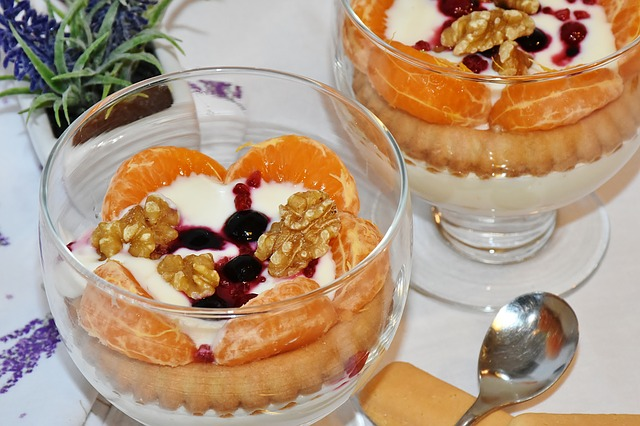
\includegraphics[width=50mm]{./images/dessert_pixabay.jpg}}
\\
(a) Original Image
\\ ~\\
\fbox{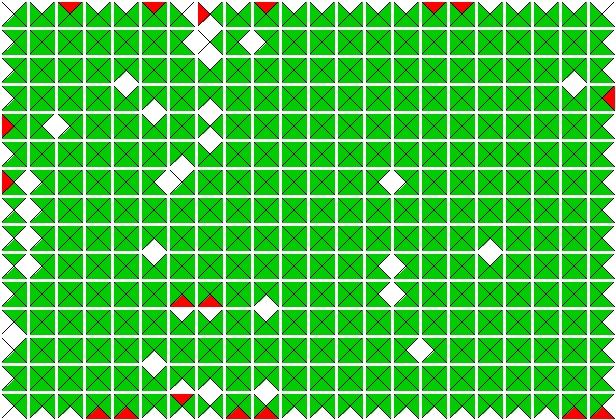
\includegraphics[width=50mm]{./images/dessert_best_buddy_visualization.jpg}}
\\
(b) Best Buddy Visualization
\caption{Visualization of Best Buddies in an Image}
\label{fig:bestBuddyVisualization}
\end{figure}

\subsubsection{Unique Best Buddies}\label{sec:improvedBestBuddies}

As explained in Section~\ref{sec:hammoudehPairwiseAffinity}, reconstructing computer generated or computer manipulated image may introduce new challenges not found with photographs; best buddies is another example of this.

In photographs, it is generally unlikely that there will be a significant number of cases where a piece has multiple best buddies on the same side.  However, computer generated images may have areas of truly solid colors, and any pieces in those areas will all be best buddies with one another, making best buddies a far less discerning indicator of compatibility.  This thesis addresses such issues by modifying the definition of best buddies as shown in Equation~\eref{eq:hammoudehBestBuddyDefinition}.

\begin{equation} \label{eq:hammoudehBestBuddyDefinition}
\begin{split}
\begin{matrix}
\forall{x_k} \forall{s_k} \in Parts, & C(x_i, s_i, x_j, s_j) > C(x_i, s_i, x_k, s_k)
\\
\\
\multicolumn{2}{c}{\textnormal{and}}
\\
\\
\forall{x_k} \forall{s_k} \in Parts, & C(x_j, s_j, x_i, s_i) > C(x_j, s_j, x_k, s_k)
\end{matrix}
\end{split}
\end{equation}

Rather than relying on best buddies being ``greater than or equal'' to all other pieces, the modified requirement is that pairings must be strictly greater than.  Hence, best buddy pairings are exclusive with cliques of size greater than two being explicitly disallowed.

\subsubsection{Interior and Exterior Best Buddies}\label{sec:interiorExteriorBestBuddies}

In all previous research, all best buddies (in particular best buddy errors) were treated the same.  However, pieces that are on the exterior (i.e. edge) of a puzzle or that are next to a missing piece are expected to naturally have a higher rate of non-adjacent best buddies than pieces on the interior of the puzzle.  This is because such piece sides do not have an true neighbor leaving them more likely to couple with an unrelated piece.  As an example, Figure~\ref{fig:bestBuddyVisualization} has four non-adjacent interior best buddies and 14 exterior non-adjacent best buddies despite there being despite there being 16 times more interior edges than exterior edges. 

When using best buddy accuracy as an estimation metric, this thesis differentiates between interior and exterior best buddy errors by giving interior best buddy errors higher weight.






%%%%%%%%%%%%%%%%%%%%%%%%%%%%%%%%%%%%%%%%%%%%%%%%%%%%%%%%%%%%%%%%%
%        Quantifying Solver Output Quality Section              %
%%%%%%%%%%%%%%%%%%%%%%%%%%%%%%%%%%%%%%%%%%%%%%%%%%%%%%%%%%%%%%%%%

\pagebreak
\section{Quantifying the Quality of a Solver Output}\label{sec:quantifyingSolverQuantify}

Cho \textit{et. al.} \cite{cho2010} defined the two metrics for quantifying the accuracy of a solver result namely: Direct Accuracy and Neighbor Accuracy. These metrics have been used in subsequent work \cite{sholomon2013, pomeranz2011, paikin2015, son2014, gallagher2012}.  This section describes the existing metrics, the weaknesses of these metrics, and proposes enhancements to these metrics to make them more meaningful for type 2 puzzles as well as when solving multiple puzzles simultaneously.

In the final subsection, tools developed to visualize the different solver quality metrics are discussed.

\subsection{Direct Accuracy}\label{sec:directAccuracy}

Direct accuracy is the most naive accuracy measure.  It is defined as the ratio of the number of pieces placed in the same location as the ground-truth (i.e. source).  The formal definition of direct accuracy ($DA$) is shown in Equation~\eref{eq:directAccuracy} where $n$ is the number of pieces in the source puzzle and $c$ is the number of pieces placed in their correct location.

\begin{equation} \label{eq:directAccuracy}
DA = \frac{c}{n}
\end{equation}

Direct accuracy is vulnerable to shifts in the solved image where even a few misplaced pieces can cause a significant decrease in the accuracy.  This can be particularly true when the ground-truth image's puzzle dimensions are not known/fixed as described in Section~\ref{sec:shiftableEnhancedDirectAccuracy}.

This thesis proposes two modifications to the direct accuracy metric known as ``Enhanced Direct Accuracy Score'' and ``Shiftable Enhanced Direct Accuracy Score''.  They each described in the following two subsections; afterwards, the thesis describes why both metrics serve complementary roles.

\subsubsection{Enhanced Direct Accuracy Score}\label{sec:enhancedDirectAccuracyScore}

The standard direct accuracy metric does not account for the possibility that in the solver output there may be pieces from multiple puzzles.  For a puzzle $P_i$ in the set of input puzzles $P$ (where $P_i \in P$) and a set of solved puzzles $S$ where $S_j$ is a solved puzzle in $S$, then Equation~\ref{eq:enhancedDirectAccuracyScore} defines the Enhanced Direct Accuracy Score (EDAS).

\begin{equation} \label{eq:enhancedDirectAccuracyScore}
EDAS_{P_i} = \argmax_{S_j \in S}\frac{c_{i,j}}{n_i + \sum_{k \ne i}(m_{k,j})}
\end{equation}

$c_{ij}$ is the number of pieces from input puzzle $P_i$ correctly placed (with no rotation in type 2 puzzles) in solved puzzle $S_j$ while $n_i$ is the number of pieces in puzzle $P_i$. $m_{k,j}$ is the number of pieces from an input puzzle $P_k$ (where $k \ne i$) that are also in solved $S_j$.

By dividing by the total number of pieces $n_i$ in puzzle $P_i$, EDAS necessarily marks as incorrect any pieces from $P_i$ that are not in solved puzzle $S_j$.  In addition, EDAS also penalizes any pieces not from $P_i$ that are in $S_j$ through the term $m_{k,j}$.  Hence, the combination of these two factors ensures that EDAS accounts both for extra and misplaced pieces.

When solving only a single puzzle, EDAS and the standard Direct Accuracy proposed by Cho \textit{et. al.} are equivalent.  In the case of solving multiple puzzles simultaneously, EDAS considers all pieces from the input puzzle of interest ($P_i$) while penalizing for pieces that are present from other input puzzles ($P_k$). 

It is important note that EDAS is a score and not a measure of accuracy. While its value is bounded between 0 and 1 (inclusive), it is not specifically defined as the number of correct placements divided by the total number of placements since the denominator may be greater than the number of pieces in the solved puzzle $S_j$.

\subsubsection{Shiftable Enhanced Direct Accuracy Score}\label{sec:shiftableEnhancedDirectAccuracy}

As mentioned previously, direct accuracy is vulnerable to shifts in the original image.  At times, the degree to which direct accuracy punishes shifts can be overly punitive. 

Figure~\ref{fig:directAccuracyOnePieceEffect} shows an original image and an actual solver output where the puzzle boundaries where not fixed.  Note that only a single piece is misplaced, causing all pieces to be shifted to the right one location.  This single misplaced piece causes the direct accuracy score to drop to 0\%.  Had this same piece been misplaced at either the right or bottom side of the image, the direct accuracy would have been largely unaffected.  The fact that direct accuracy can give such vastly differing results for essentially the same error indicates that it has room for improvement.

\begin{figure}
\centering
\fbox{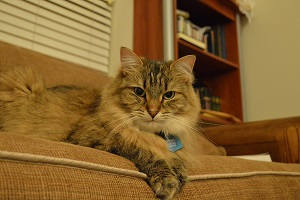
\includegraphics[width=50mm]{./images/muffins_300x200.jpg}}
\\
(a) Original Image
\\ ~\\
\fbox{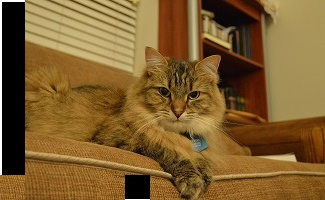
\includegraphics[width=54.17mm]{./images/muffins_300x200_type1}}
\\
(b) Solver Output
\caption{Solver Output where a Single Misplaced Piece Catastrophically Affects the Direct Accuracy}
\label{fig:directAccuracyOnePieceEffect}
\end{figure}

To address the often misleadingly punitive nature of the direct accuracy measure, this thesis proposes the Shiftable Enhanced Direct Accuracy Score (SEDAS).  Let $p_n$ be the puzzle piece that is closest to the upper left corner of the solved image's boundary with a minimum Manhattan distance $d_min$.  Also let $L$ as the set of all possible puzzle piece locations that minimum distance $d_min$, then the SEDAS for a puzzle $P_i$ is defined as:

\begin{equation} \label{eq:shiftableEnhancedDirectAccuracyScore}
SEDAS_{P_i} = \argmax_{l \in L} \Big( \argmax_{S_j \in S}\frac{c_{i,j,l}}{n_i + \sum_{k \ne i}(m_{k,j})} \Big)
\end{equation}

Note that as reference point ($l$) for the solved is shifted, then only the number of pieces in the correct location ($c_{i,j,l}$) will also change.  

Rather than defining SEDAS based off the closest puzzle to the upper left corner of the image, an alternative is to use the point anywhere in the image that maximizes Equation~\eref{eq:shiftableEnhancedDirectAccuracyScore}.  However, that approach will usually be significantly more computationally complex in particular on large puzzles of several thousand pieces.  Hence, this thesis' approach balances finding a meaningful direct accuracy score with computational efficiency.

\subsubsection{Importance of Using Both EDAS and SEDAS}\label{sec:importanceEdasSedas}

While EDAS can be misleadingly punitive, it is not correct that EDAS should be wholly replaced by SEDAS.  Rather, EDAS and SEDAS serve complementary roles.  First, EDAS must necessarily be calculated as part of SEDAS since the upper left corner location is inherently a member of the set of minimum distance locations ``$L$'' (as defined in Equation~\eref{eq:shiftableEnhancedDirectAccuracyScore}).  Hence, there is no additional computational time required to calculate EDAS.  What is more, by continuing to use EDAS along with SEDAS, it is often possible to detect whether there was any shifting in the original image.  This would not be possible if SEDAS was used alone.

\subsection{Neighbor Accuracy}\label{sec:neighborAccuracy}

Cho \textit{et. al.} \cite{cho2010} defined neighbor accuracy as the ratio of the number of puzzle piece sides adjacent to the same piece's side in the ground-truth image as in the solved image over the total number of piece sides.  More formally, let $q$ be the number of sides of each puzzle piece (i.e. 4), and $n$ be the number of pieces in the original.  If $a$ is the number of puzzle piece sides adjacent in the ground-truth and solved images, then the neighbor accuracy ($NA$) is defined as shown in Equation~\eref{eq:neighborAccuracy}.

\begin{equation} \label{eq:neighborAccuracy}
NA = \frac{a}{n~q}
\end{equation}

Unlike direct accuracy, neighbor accuracy is largely unaffected by shifts in the solved image since it considers a piece's neighbors and not its actual location.  However, it does not define how to handle the presence of pieces from multiple puzzles in the solved result.  Therefore, it must be amended to consider such cases.

\subsection{Enhanced Neighbor Accuracy Score}\label{sec:enhancedNeighborAccuracyScore}

Similar to EDAS for Direct Accuracy, Enhanced Neighbor Accuracy Score (ENAS) addresses neighbor accuracy's limitations when quantifying the quality of a solver output when solving multiple puzzles simultaneously. 

Let $n_i$ be the number of puzzles pieces in the input puzzle $P_i$ and $a_{i,j}$ be the number of puzzle piece sides in puzzle $P_i$ that are adjacent in solved puzzle $S_j$.  If $m_{k,j}$ is the number of puzzle pieces from an input puzzle $P_k$ (where $k \ne i$) in $S_j$, then the Enhanced Neighbor Accuracy Score for $P_i$ is defined in Equation~\eref{eq:enhancedNeighborAccuracyScore}.

\begin{equation} \label{eq:enhancedNeighborAccuracyScore}
ENAS_{P_i} = \argmax_{S_j \in S}\frac{a_{i,j}}{q ~ (n_i + \sum_{k \ne i}(m_{k,j})}
\end{equation}

Similar to EDAS as described in Section~\ref{sec:enhancedDirectAccuracyScore}, ENAS divides by the number of pieces $n_i$ in input puzzle $P_i$.  By doing so, it effectively marks as incorrect any pieces from $P_i$ not in $S_j$.  What is more, by including in the summation in the denominator of \eref{eq:enhancedNeighborAccuracyScore}, ENAS marks as necessarily incorrect any pieces not from $P_i$ that are in $S_j$.  The combination of these two factors allow ENAS to account for extra and misplaced pieces.

\subsection{Visualizing Solver Accuracy Results}\label{sec:visualizingSolverAccuracy}

In images with thousands of pieces, it is often difficult to visually determine the location of pieces that are placed incorrectly.  What is more, visual tools help developers quickly detect and fix latent bugs that may be in their program.

The following two subsections show the tools developed as part of this thesis for visualizing direct accuracy and neighbor accuracy.

\subsubsection{Visualizing EDAS and SEDAS}\label{sec:visualizingEdasSedas}

Regardless of whether standard direct accuracy, EDAS, or SEDAS is used, each puzzle piece is assigned a single value (e.g. correct or incorrect).  Due to that, the direct accuracy visualization represents each puzzle by a solid color square.  One additional refinement used is to subdivide the ``incorrect'' placements into a set of subcategories namely (in order of severity): wrong puzzle, wrong location, and wrong rotation.  Table~\ref{tab:directAccuracyColors} shows the colors assigned to puzzle pieces depending on their direct accuracy classification.

\begin{table}[h]

\begin{center}
  \begin{tabular}{ | >{\centering\arraybackslash}m{0.6in} | >{\centering\arraybackslash}m{0.6in} | >{\centering\arraybackslash}m{0.6in} | >{\centering\arraybackslash}m{0.6in} | >{\centering\arraybackslash}m{0.6in} | }
 \hline
    Wrong Puzzle & Wrong Location & Wrong Rotation & Correct Location  & No Piece Present  \\ \hline
	{\cellcolor{blue}~} & {\cellcolor{red}~}  & {\cellcolor{orange}~}  & {\cellcolor{green}~} & {\cellcolor{black}~}  \\
	{\cellcolor{blue}~} & {\cellcolor{red}~}  & {\cellcolor{orange}~}  & {\cellcolor{green}~} & {\cellcolor{black}~} \\
 \hline
  \end{tabular}
\end{center}
\caption{Coloring Definition for Pieces in the Direct Accuracy Solver Output Visualization}\label{tab:directAccuracyColors}
\end{table}

Figure~\ref{fig:directAccuracyVisualization} shows a solver output along with the EDAS and SEDAS visualizations. Since four puzzle pieces were erroneously placed on the left of the image, almost all pieces had the wrong location according to EDAS; the only exception is a single piece that had the right location, but wrong rotation.  In contrast, almost all pieces had the correct location in the SEDAS representation; note that the piece that previously had the correct location but wrong rotation in EDAS has the wrong location in SEDAS.

\begin{figure}
\centering

  \begin{tabular}{ >{\centering\arraybackslash}m{2.2in} >{\centering\arraybackslash}m{2.2in} }
  
	\fbox{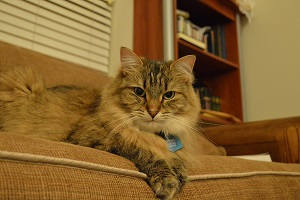
\includegraphics[width=48mm]{./images/muffins_300x200.jpg}} & \fbox{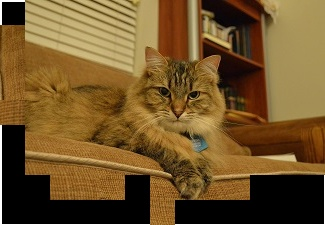
\includegraphics[width=52.1mm]{./images/muffins_300x200_type2}} \\~\\
	(a) Ground-Truth Image & (b) Type 2 Solver Output
\\~\\
	\fbox{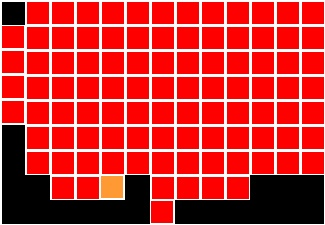
\includegraphics[width=52.1mm]{./images/muffins_300x200_type_EDAS.jpg}} & \fbox{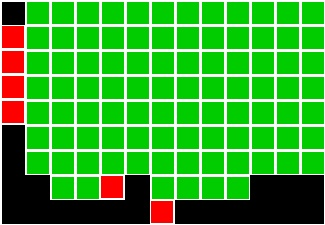
\includegraphics[width=52.1mm]{./images/muffins_300x200_type_SEDAS.jpg}}
\\~\\
	(c) EDAS Visualization & (d) SEDAS Visualization  
  \end{tabular}

\caption{Example Solver Output Visualizations for EDAS and SEDAS}
\label{fig:directAccuracyVisualization}
\end{figure}

\subsubsection{Visualizing Neighbor Accuracy}\label{sec:visualizingNeighborAccuracy}

The visualization for neighbor accuracy is very similar to the techniques described in Section~\ref{sec:visualizingBestBuddies} for visualizing best buddies.  Each puzzle piece is divided into four equal-sized isosceles triangles (i.e. one for each side).  The triangles are assigned colors depending on whether their neighbor in the solver output matches their neighbor in the ground-truth image.  The visualization includes a subcategory known as ``wrong puzzle'' which is a special case that occurs when solving multiple puzzles simultaneously and some of the pieces in the solved puzzle are not from the puzzle of interest (i.e. $P_i$).  Table~\ref{tab:neighborAccuracyColors} defines the colors used to represent the different classification of puzzle piece sides for neighbor accuracy.

\begin{table}[h]
\begin{center}
  \begin{tabular}{ | >{\centering\arraybackslash}m{0.6in} | >{\centering\arraybackslash}m{0.6in} | >{\centering\arraybackslash}m{0.6in} | >{\centering\arraybackslash}m{0.6in} | >{\centering\arraybackslash}m{0.6in} | }
 \hline
    Wrong Puzzle & Wrong Neighbor & Correct Neighbor  & No Piece Present  \\ \hline
	{\cellcolor{blue}~} & {\cellcolor{red}~} & {\cellcolor{green}~} & {\cellcolor{black}~}  \\
	{\cellcolor{blue}~} & {\cellcolor{red}~} & {\cellcolor{green}~} & {\cellcolor{black}~}  \\
 \hline
  \end{tabular}
\end{center}
\caption{Coloring Definition for Puzzle Piece Sides in the Neighbor Accuracy Solver Output Visualization}\label{tab:neighborAccuracyColors}
\end{table}

Figure~\ref{fig:neigborAccuracyVisualization} shows the output when solving two images simultaneously.  Note that one of the input puzzles is a rainforest scene while the other is building exterior.  In this case the puzzle of interest was the rainforest image.  

\begin{figure}
\centering

  \begin{tabular}{ >{\centering\arraybackslash}m{2.2in} >{\centering\arraybackslash}m{2.2in} }
  
	\fbox{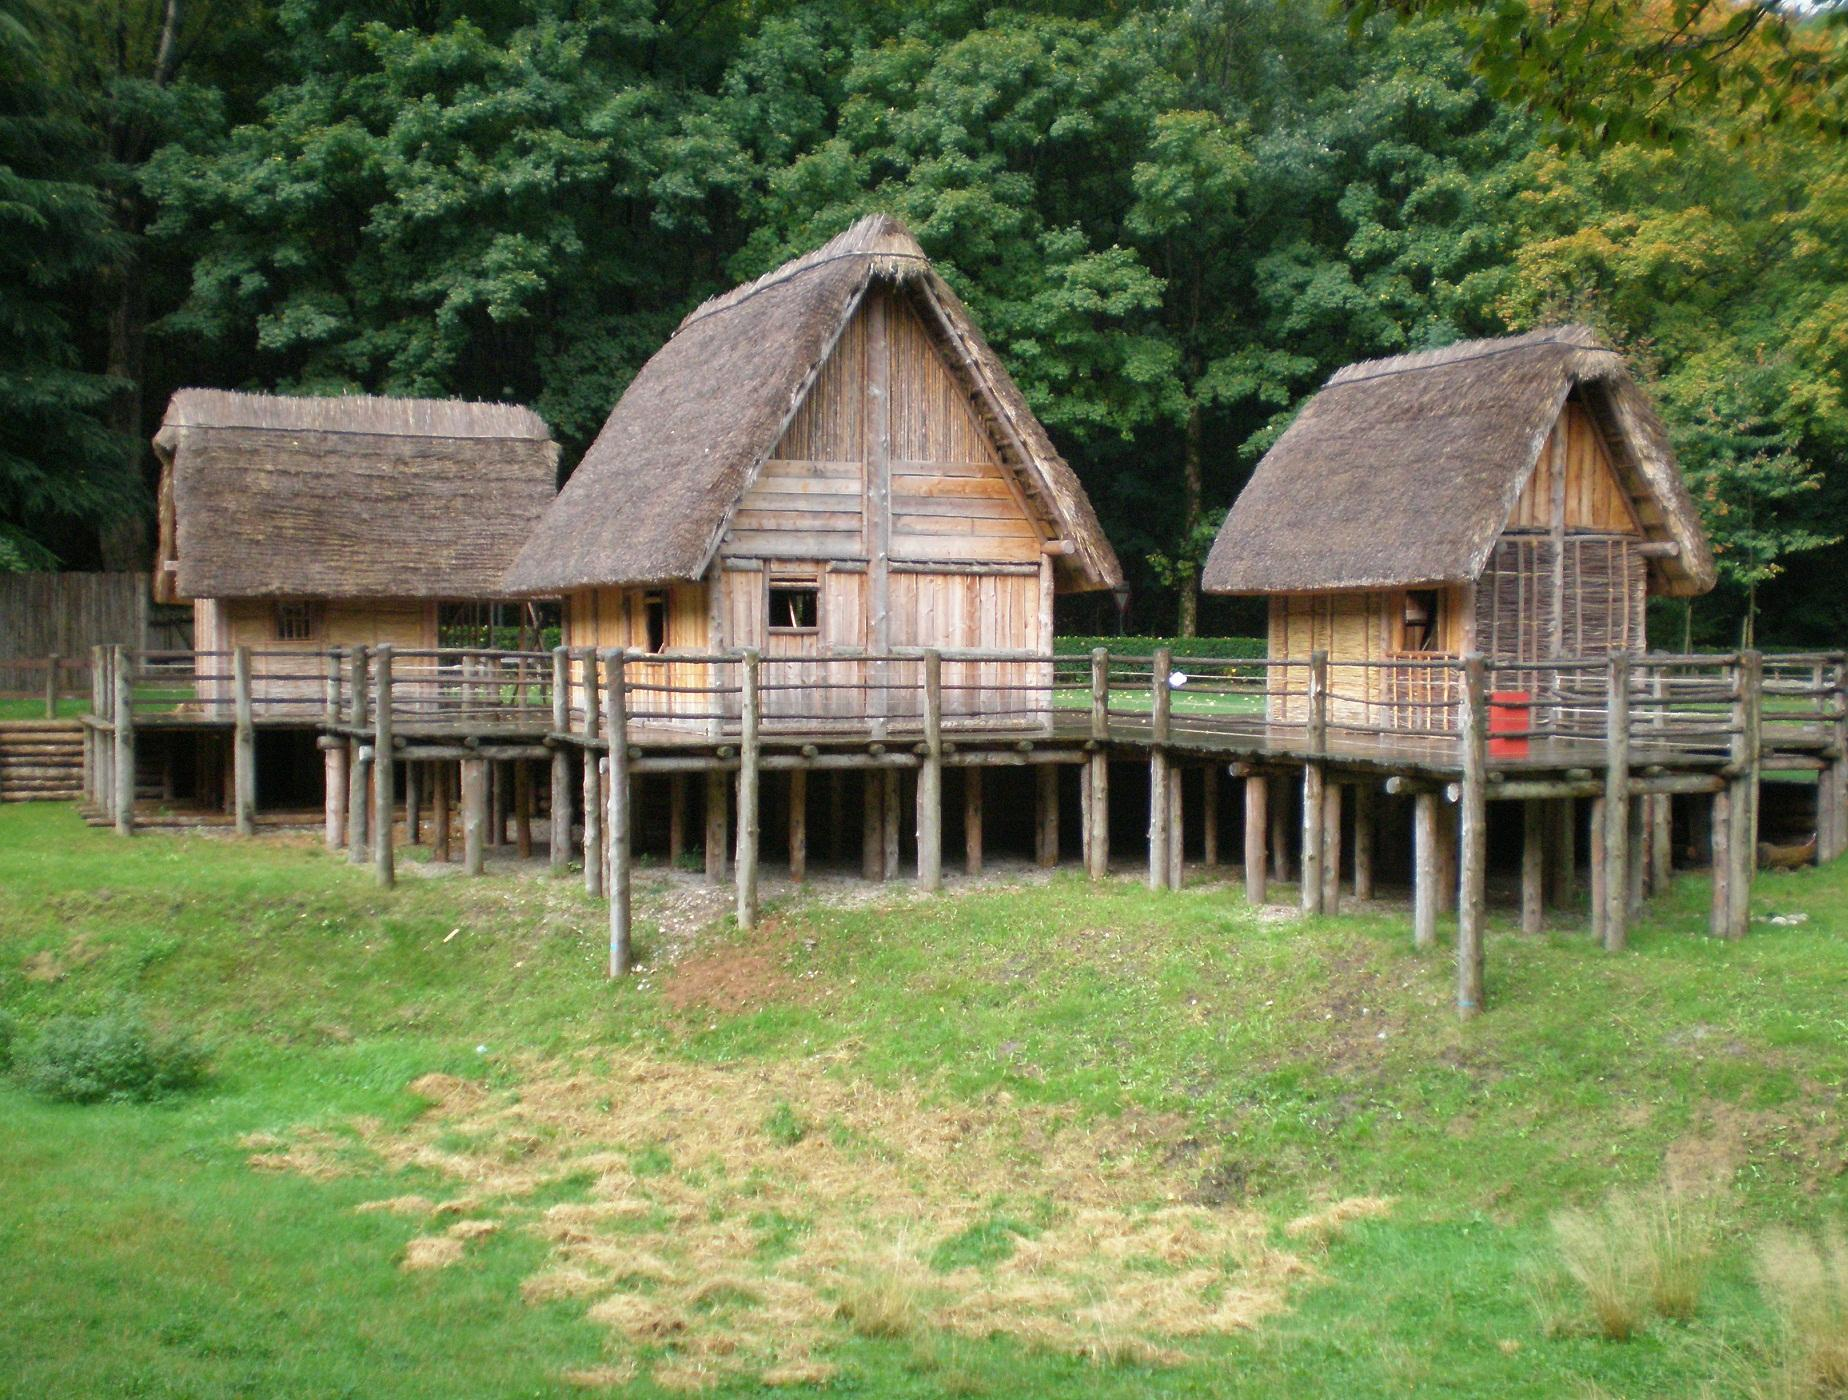
\includegraphics[width=1.75in]{./images/pomeranz_3300_1.jpg}} & \fbox{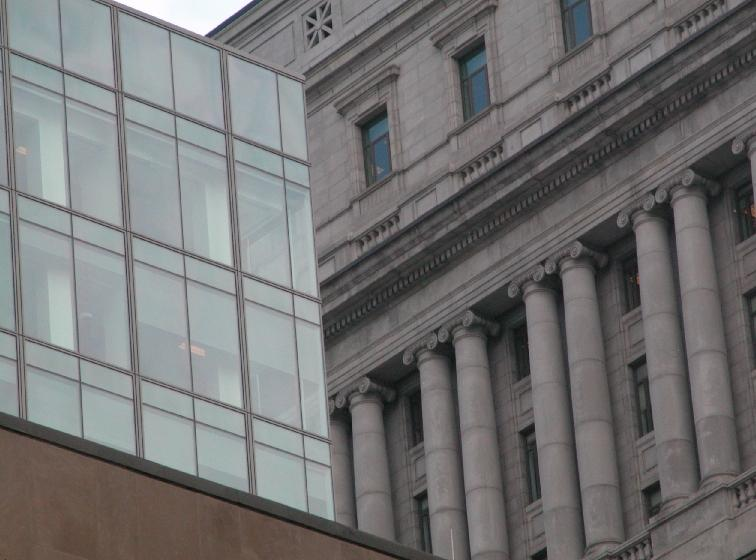
\includegraphics[width=1.5in]{./images/mcgill_20.jpg}} \\~\\
	(a) Input Image \# 1 - Rainforest House \cite{pomeranzBenchmarkImages} & (b) Input Image \# 2 - Building Exterior \cite{mcgillImageDatabase}
\\~\\
	\fbox{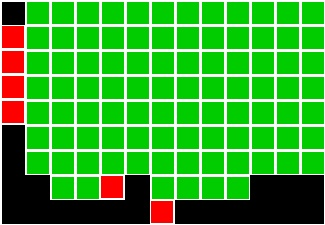
\includegraphics[width=50mm]{./images/muffins_300x200_type_SEDAS.jpg}}
	& \fbox{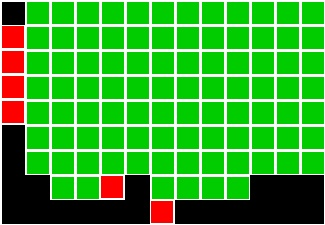
\includegraphics[width=50mm]{./images/muffins_300x200_type_SEDAS.jpg}}
\\~\\
	(c) Solver Output & (d) ENAS Visualization  
  \end{tabular}

\caption{Example Solver Output Visualization for ENAS}
\label{fig:neigborAccuracyVisualization}
\end{figure}

All pieces that came from the building exterior image are shown as blue.  The pieces from the ''rainforest house'' image that are adjacent to the other image's pieces are shown in as red since they come from the puzzle of interest but have the wrong neighbor.








%%%%%%%%%%%%%%%%%%%%%%%%%%%%%%%%%%%%%%%%%%%%%%%%%%%%%%%%%%%%%%%%%
%                    Paikin & Tal Solver                        %
%%%%%%%%%%%%%%%%%%%%%%%%%%%%%%%%%%%%%%%%%%%%%%%%%%%%%%%%%%%%%%%%%

\pagebreak
\section{Paikin \& Tal Solver}\label{sec:paikinTalSolver}

This section reviews the solver proposed by Paikin \& Tal \cite{paikin2015}; their Java implementation was never open sourced.  As such, this section also describes a complete implementation of their approach developed as part of this thesis.  The section concludes with a summary of some of the weaknesses of Paikin \& Tal's approach. 

\subsection{Overview of Paikin \& Tal's Algorithm}\label{sec:paikinTalAlgorithm}

Paikin \& Tal's solver was inspired by the solver developed by Pomeranz \textit{et. al.} in \cite{pomeranz2011}.  However, unlike the previous work, Paikin \& Tal's is deterministic; their greedy algorithm iteratively places the puzzle piece that at each stage has the maximum confidence score. Paikin \& Tal's approach is able to handle puzzles with missing pieces where the puzzle size and piece orientation are unknown.  The only input provided to the algorithm is the expected number of output puzzles.

Paikin \& Tal's algorithm has three distinct phases namely: inter-puzzle piece distance calculation, selecting of the seed piece, and placement.  These are described in the following subsections.  The modification required to the algorithm to solve multiple puzzles simultaneously is describing in an additional subsection.

\subsubsection{Inter-Puzzle Piece Distance Calculation}\label{sec:paikinTalInterPieceDistance}

The first stage of Paikin \& Tal's algorithm is to calculate the inter-piece distance between all pairs of pieces.  This is done using the asymmetric distance measure described in Section~\eref{eq:paikinAsymDistance}.  This information is stored in an $n$ by $n$ matrix (where $n$ is the number of puzzle pieces); after being calculated, the asymmetric distance never needs to be recalculated again throughout the duration of the algorithm.

As explained in Section~\ref{eq:paikinAsymDistance}, Paikin \& Tal normalizes all of the asymmetric distances between each possible pairing of pieces by the second best distance for each piece.  This has the effect of amplifying truly unique pairings versus pairings that arise from low variation areas of the image.  They refer to this as ``asymmetric compatibility''.  The asymmetric compatibility is then used to find the best buddies (if any) for all pieces.  

The last step when calculating inter-piece distance is to calculate the mutual compatibility ($\tilde{C}$), which is defined in Equation~\eref{eq:mutualCompatibility}.  $C(x_i,s_i,x_j,s_j)$ is the asymmetric compatibility between side $s_i$ of piece $x_j$ and side $s_j$ of piece $x_j$; $C(x_j,s_j,x_i,s_i)$ is defined similarly.  It is important to note that mutual compatibility is symmetric.

\begin{equation} \label{eq:mutualCompatibility}
\tilde{C}(x_i,s_i,x_j,s_j)=\tilde{C}(x_j,s_j,x_i,s_i)=\frac{C(x_i,s_i,x_j,s_j) + C(x_j,s_j,x_i,s_i) }{2}
\end{equation}

\subsubsection{Selecting the Seed Piece}\label{sec:paikinTalSeedPiece}

Similar to Pomeranz \textit{et. al.}, Paikin \& Tal is a kernel growing algorithm.  Hence, a seed piece is selected, and all pieces are placed around that initial seed.    Since the algorithm is greedy, the selection of a poor seed can have a significant effect on the final solution.  Due to this, Paikin \& Tal select a piece that is itself ``distinctive'' and comes from a ``distinctive region.''  

Paikin \& Tal define a seed piece as distinctive if it has best buddies on each of its sides.  To ensure that a piece comes from a distinctive region, all of the seed piece's best buddies must also have four best buddies. In a puzzle, there may be multiple pieces that satisfy the ``distinctive'' piece in a ``distinctive region'' criteria; ties are broken by selecting the piece that has the maximum sum of mutual compatibilities among its neighbors.

\subsubsection{Placement}\label{sec:paikinTalPlacer}



\begin{algorithm}
\caption{Paikin \& Tal Placer}\label{alg:paikinTalPlacer}
\begin{algorithmic}[1]
\While{ |UnplacedPieces| > 0 }

   \If{ |BestBuddyPool| > 0 }
      \State Get best candidate from the BestBuddyPool
   \Else
      \State Recalculate the asymmetric and mutual compatibility
      \State Select piece with the highest asymmetric compatibility
   \EndIf  
   \State Place the best piece
   \State Add the placed piece's unplaced best buddies to the BestBuddyPool

\EndWhile
\end{algorithmic}
\end{algorithm}


\subsection{A Python Implementation of Paikin \& Tal's Algorithm}\label{sec:pythonPaikinTalAlgorithm}















%%%%%%%%%%%%%%%%%%%%%%%%%%%%%%%%%%%%%%%%%%%%%%%%%%%%%%%%%%%%%%%%%
%              Bibliography and Document End                    %
%%%%%%%%%%%%%%%%%%%%%%%%%%%%%%%%%%%%%%%%%%%%%%%%%%%%%%%%%%%%%%%%%

\pagebreak
\bibliographystyle{ieeetr}
\bibliography{cs297_final_report_biblio}

\end{document}
